\begin{figure}[h]
    \centering
    \begin{tabular}{cc}
        \subfloat[][$B^0 \to D(K\pi)K^{*0}$ Run 1]{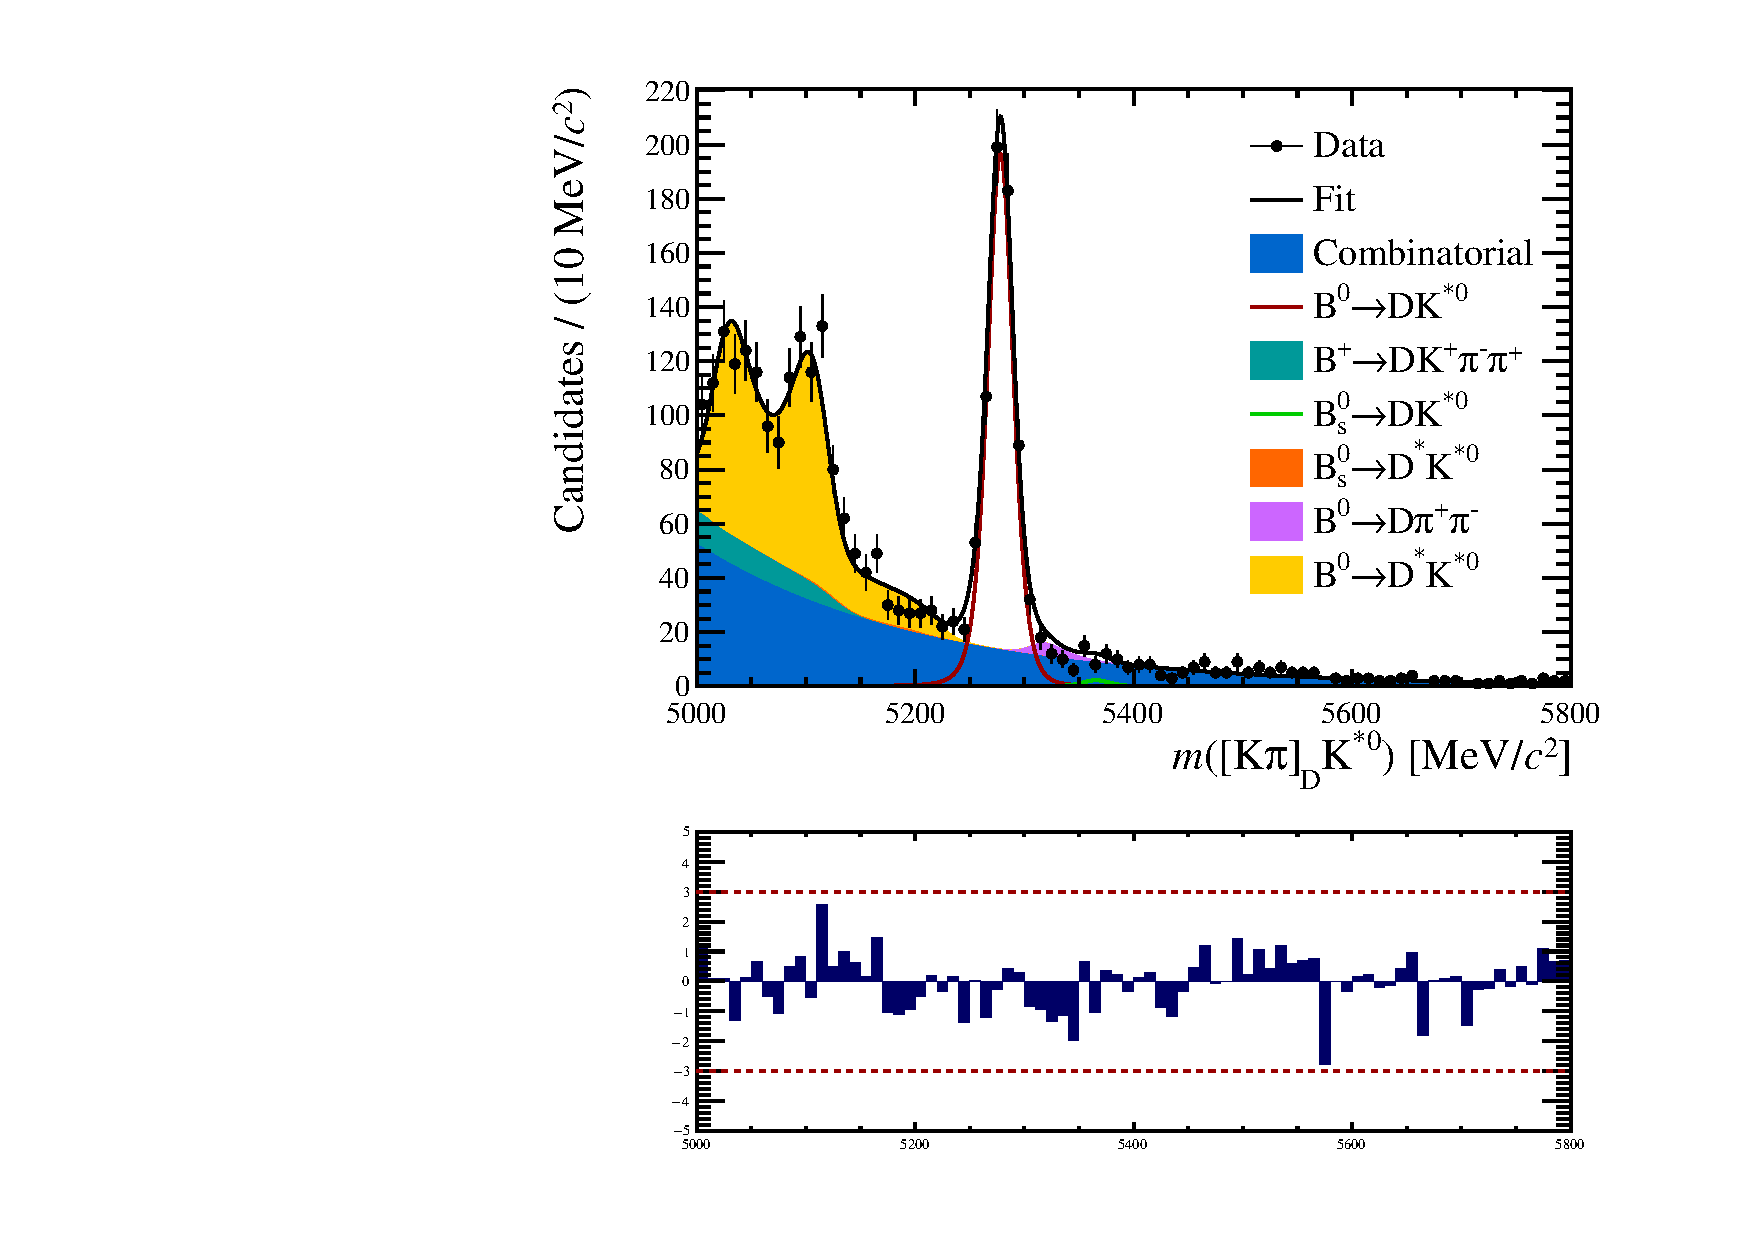
\includegraphics[width=0.45\textwidth]{ANA_resources/Plots/Data_fit/twoAndFourBody_data_Kpi_run1}} &
        \subfloat[][$B^0 \to D(K\pi)K^{*0}$ Run 2]{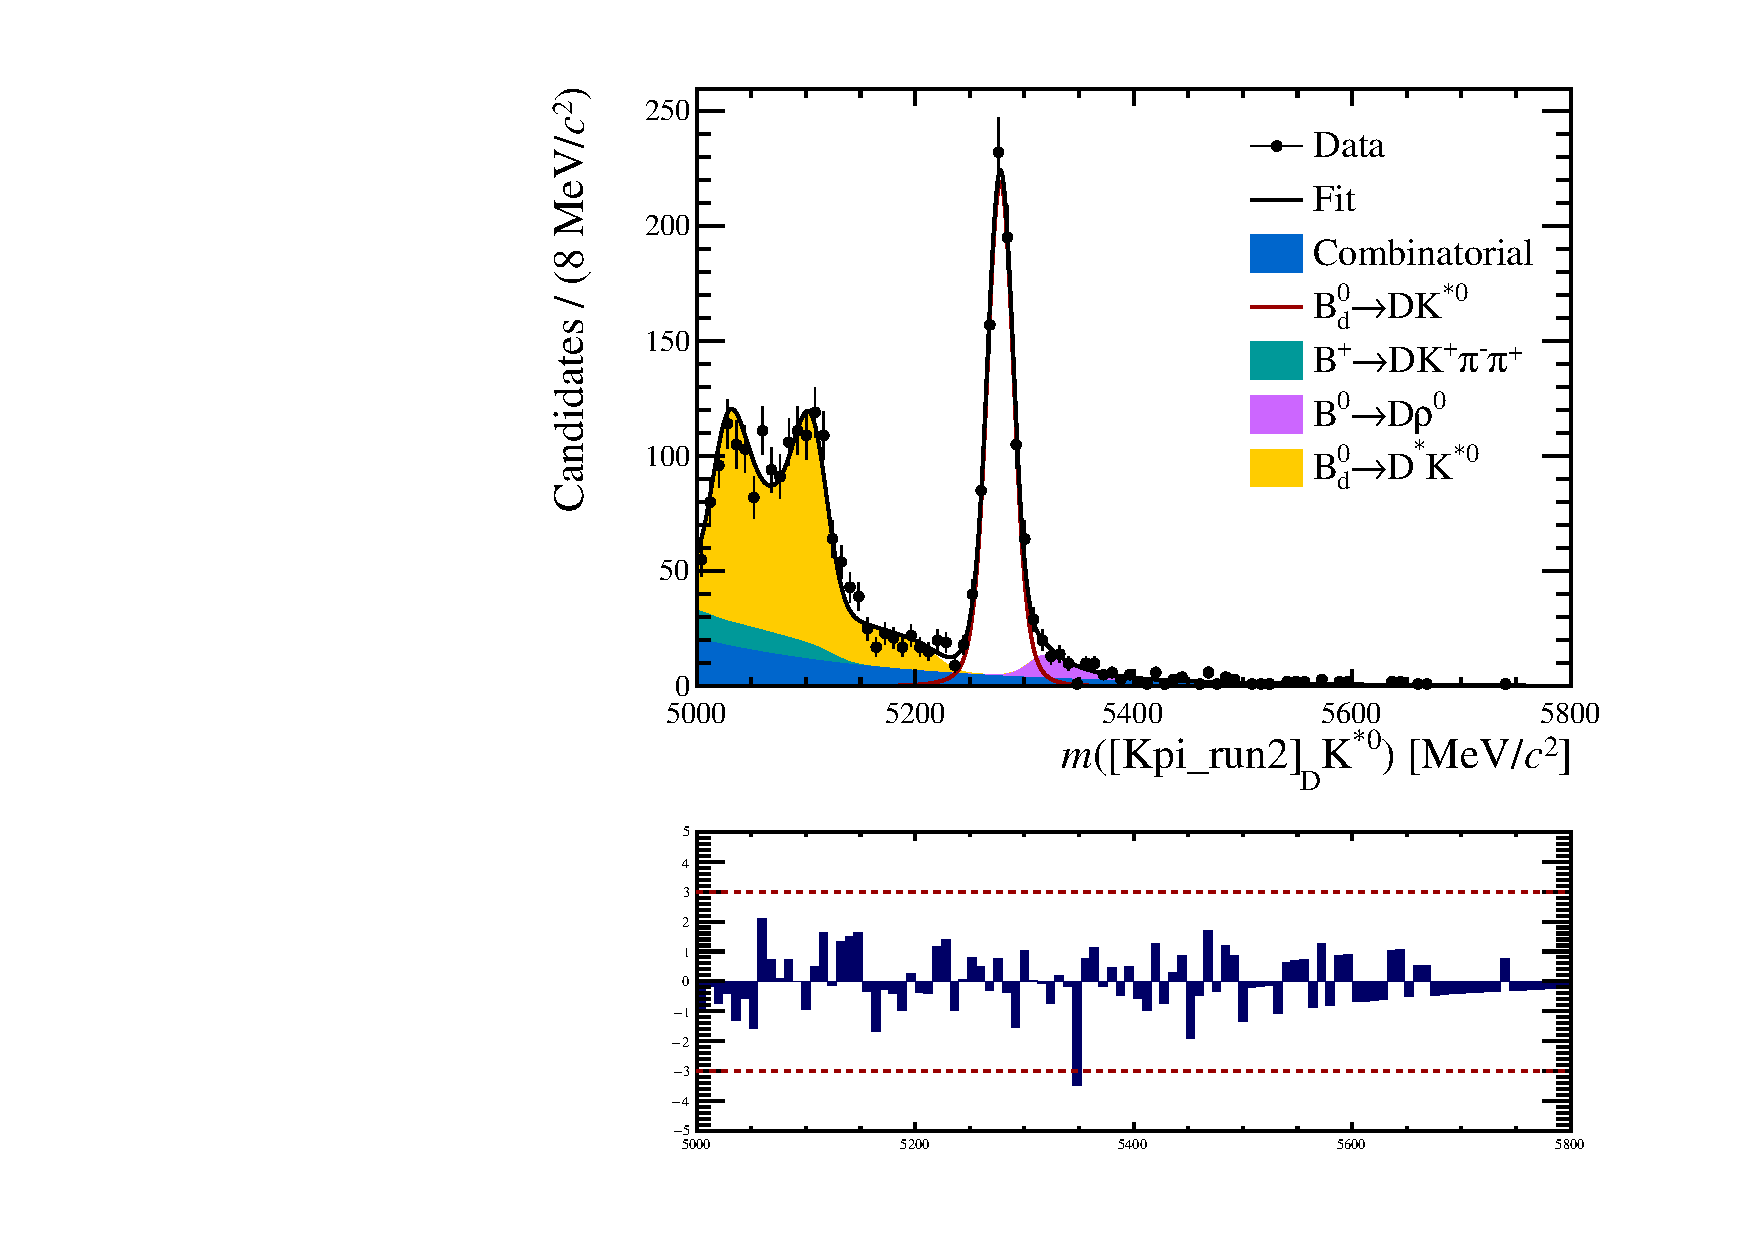
\includegraphics[width=0.45\textwidth]{ANA_resources/Plots/Data_fit/twoAndFourBody_data_Kpi_run2.pdf}} \\
    \end{tabular}
    \caption{Fit to $B$ invariant mass of selected candidates in the $K\pi$ final state, split by run and summed over $B$ flavour.}
\label{fig:data_fit_Kpi_combined}
\end{figure}
\begin{figure}[h]
    \centering
    \begin{tabular}{cc}
        \subfloat[][$B^0 \to D(\pi K)K^{*0}$ Run 1]{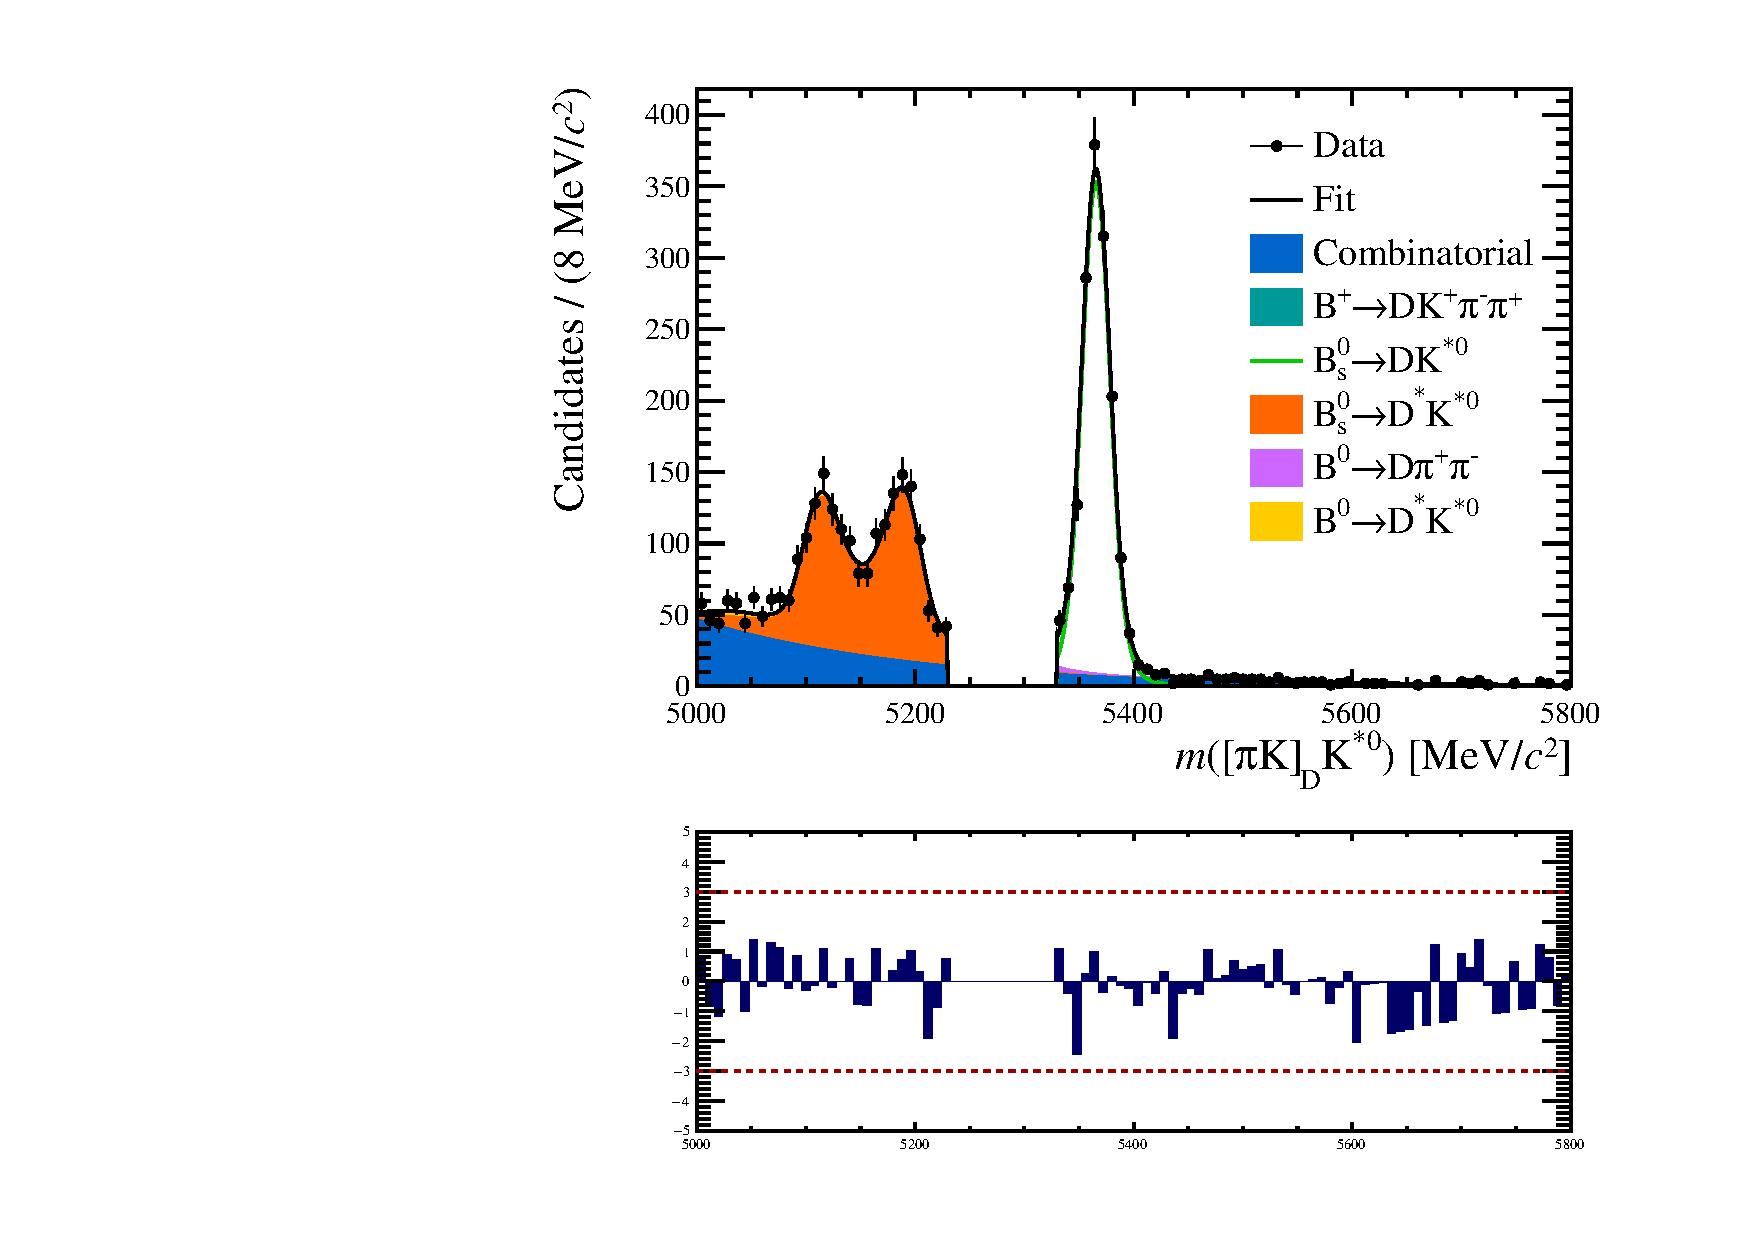
\includegraphics[width=0.45\textwidth]{ANA_resources/Plots/Data_fit/twoAndFourBody_data_piK_run1}} &
        \subfloat[][$B^0 \to D(\pi K)K^{*0}$ Run 2]{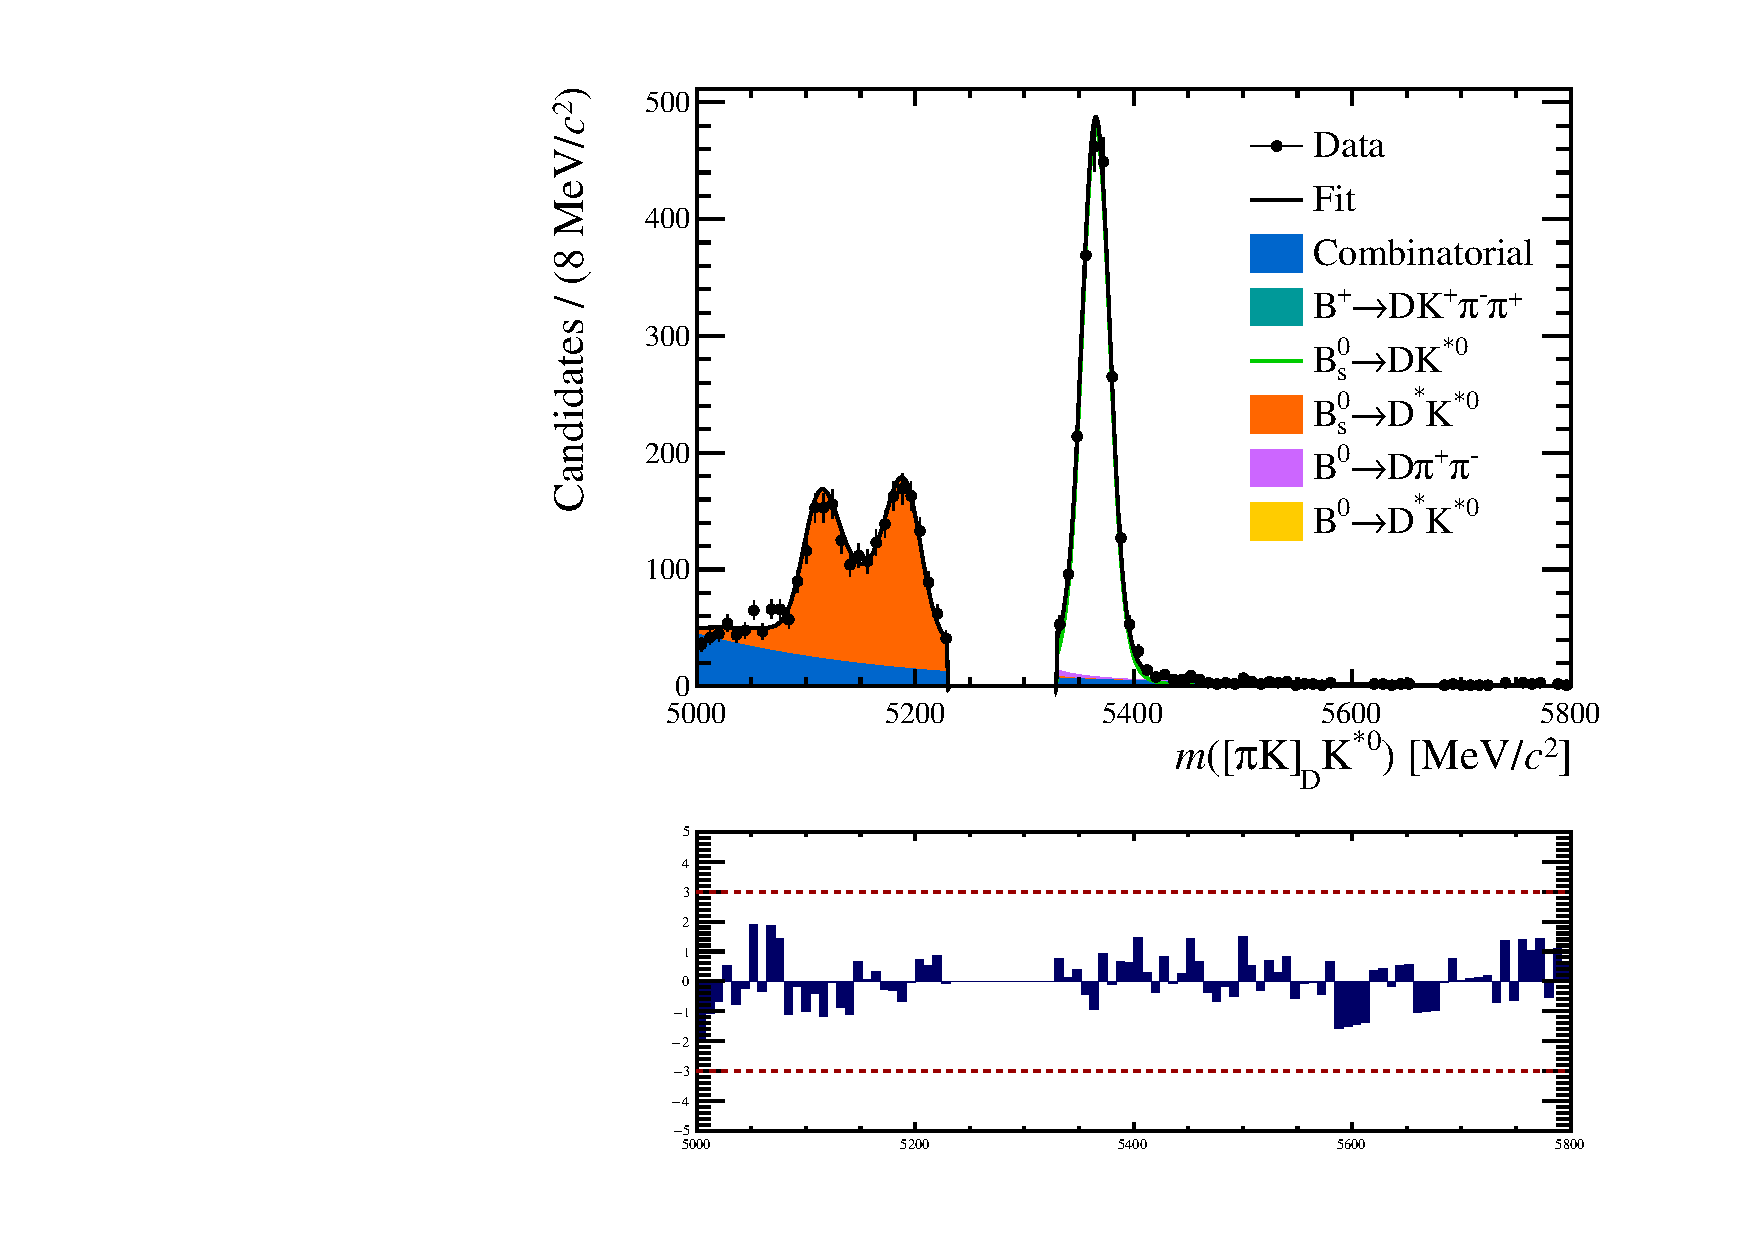
\includegraphics[width=0.45\textwidth]{ANA_resources/Plots/Data_fit/twoAndFourBody_data_piK_run2.pdf}} \\
    \end{tabular}
    \caption{Fit to $B$ invariant mass of selected candidates in the $\pi K$ final state, split by run and summed over $B$ flavour.}
\label{fig:data_fit_piK_combined}
\end{figure}
\begin{figure}[h]
    \centering
    \begin{tabular}{cc}
        \subfloat[][$B^0 \to D(KK)K^{*0}$ Run 1]{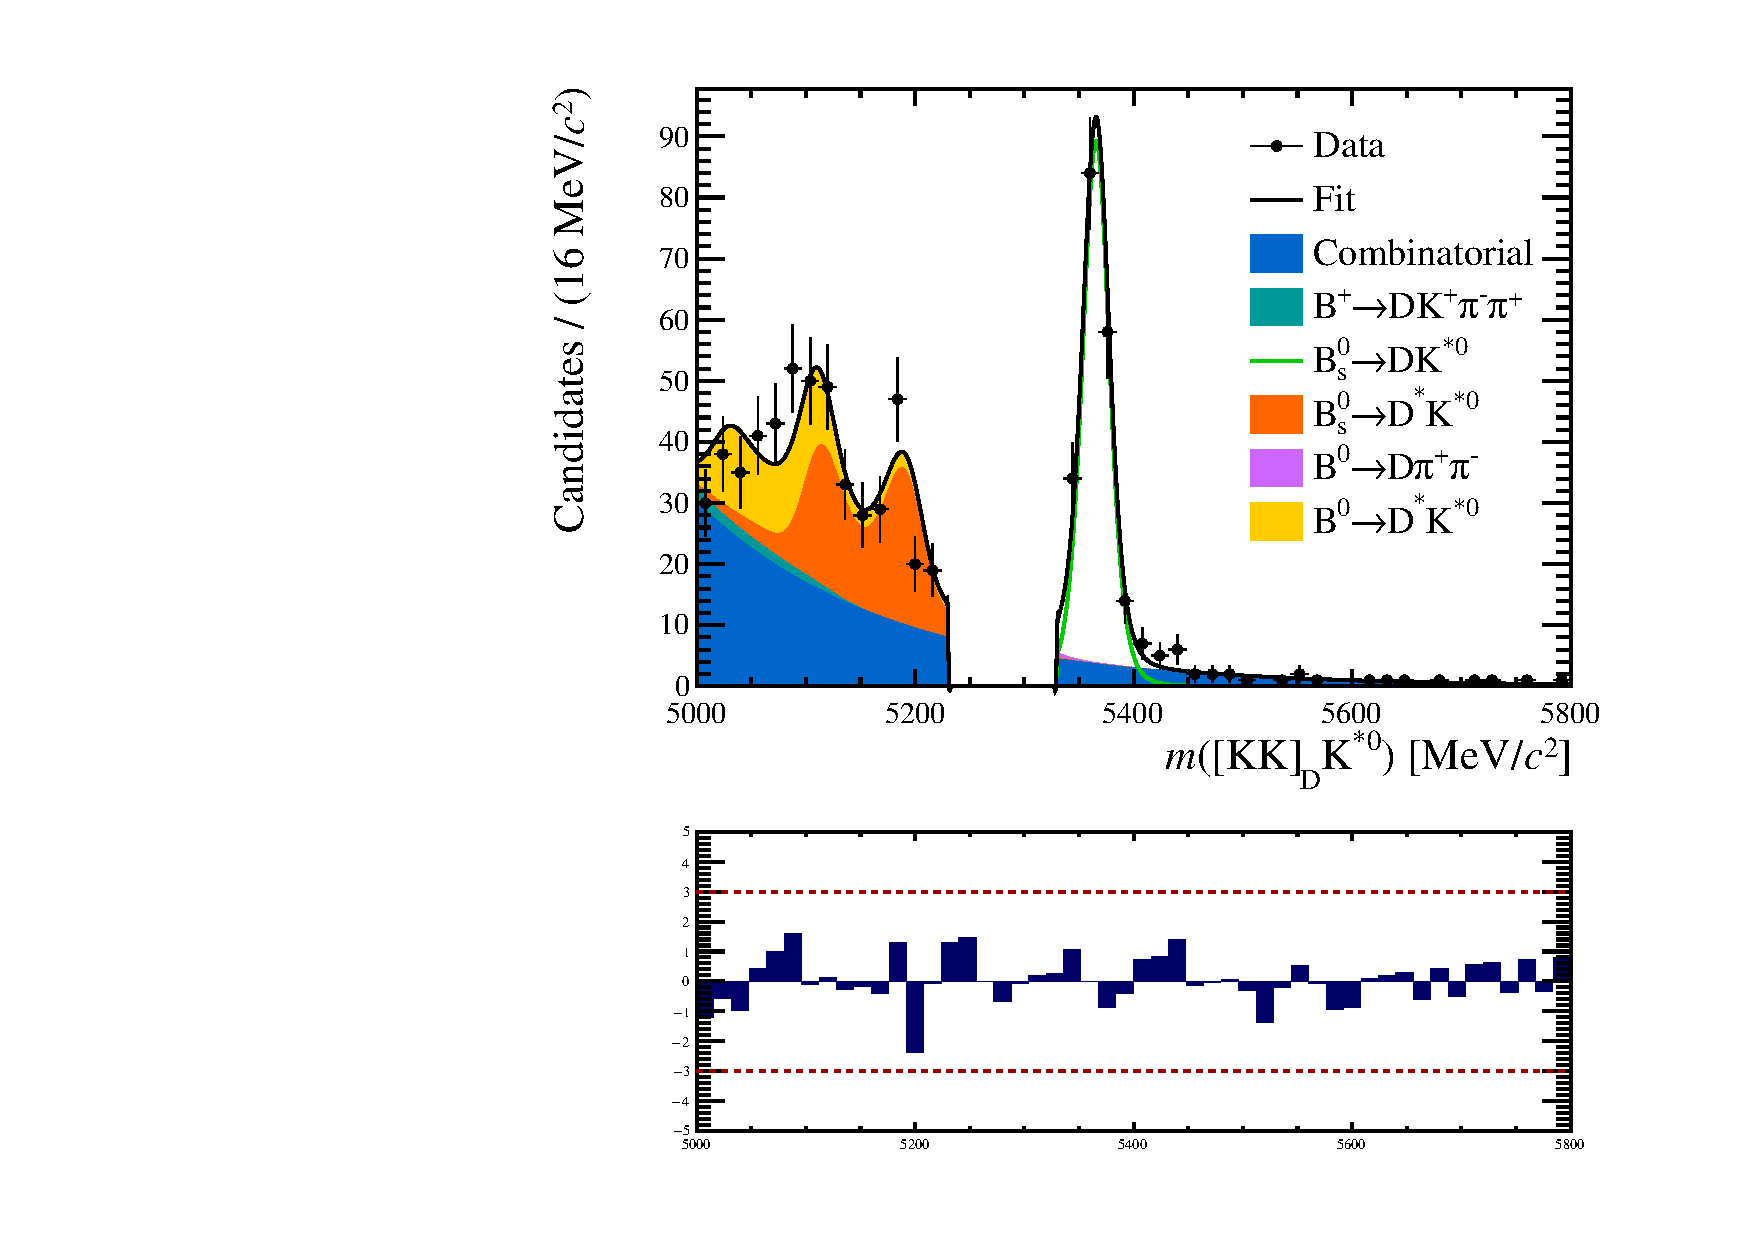
\includegraphics[width=0.45\textwidth]{ANA_resources/Plots/Data_fit/twoAndFourBody_data_KK_run1}} &
        \subfloat[][$B^0 \to D(KK)K^{*0}$ Run 2]{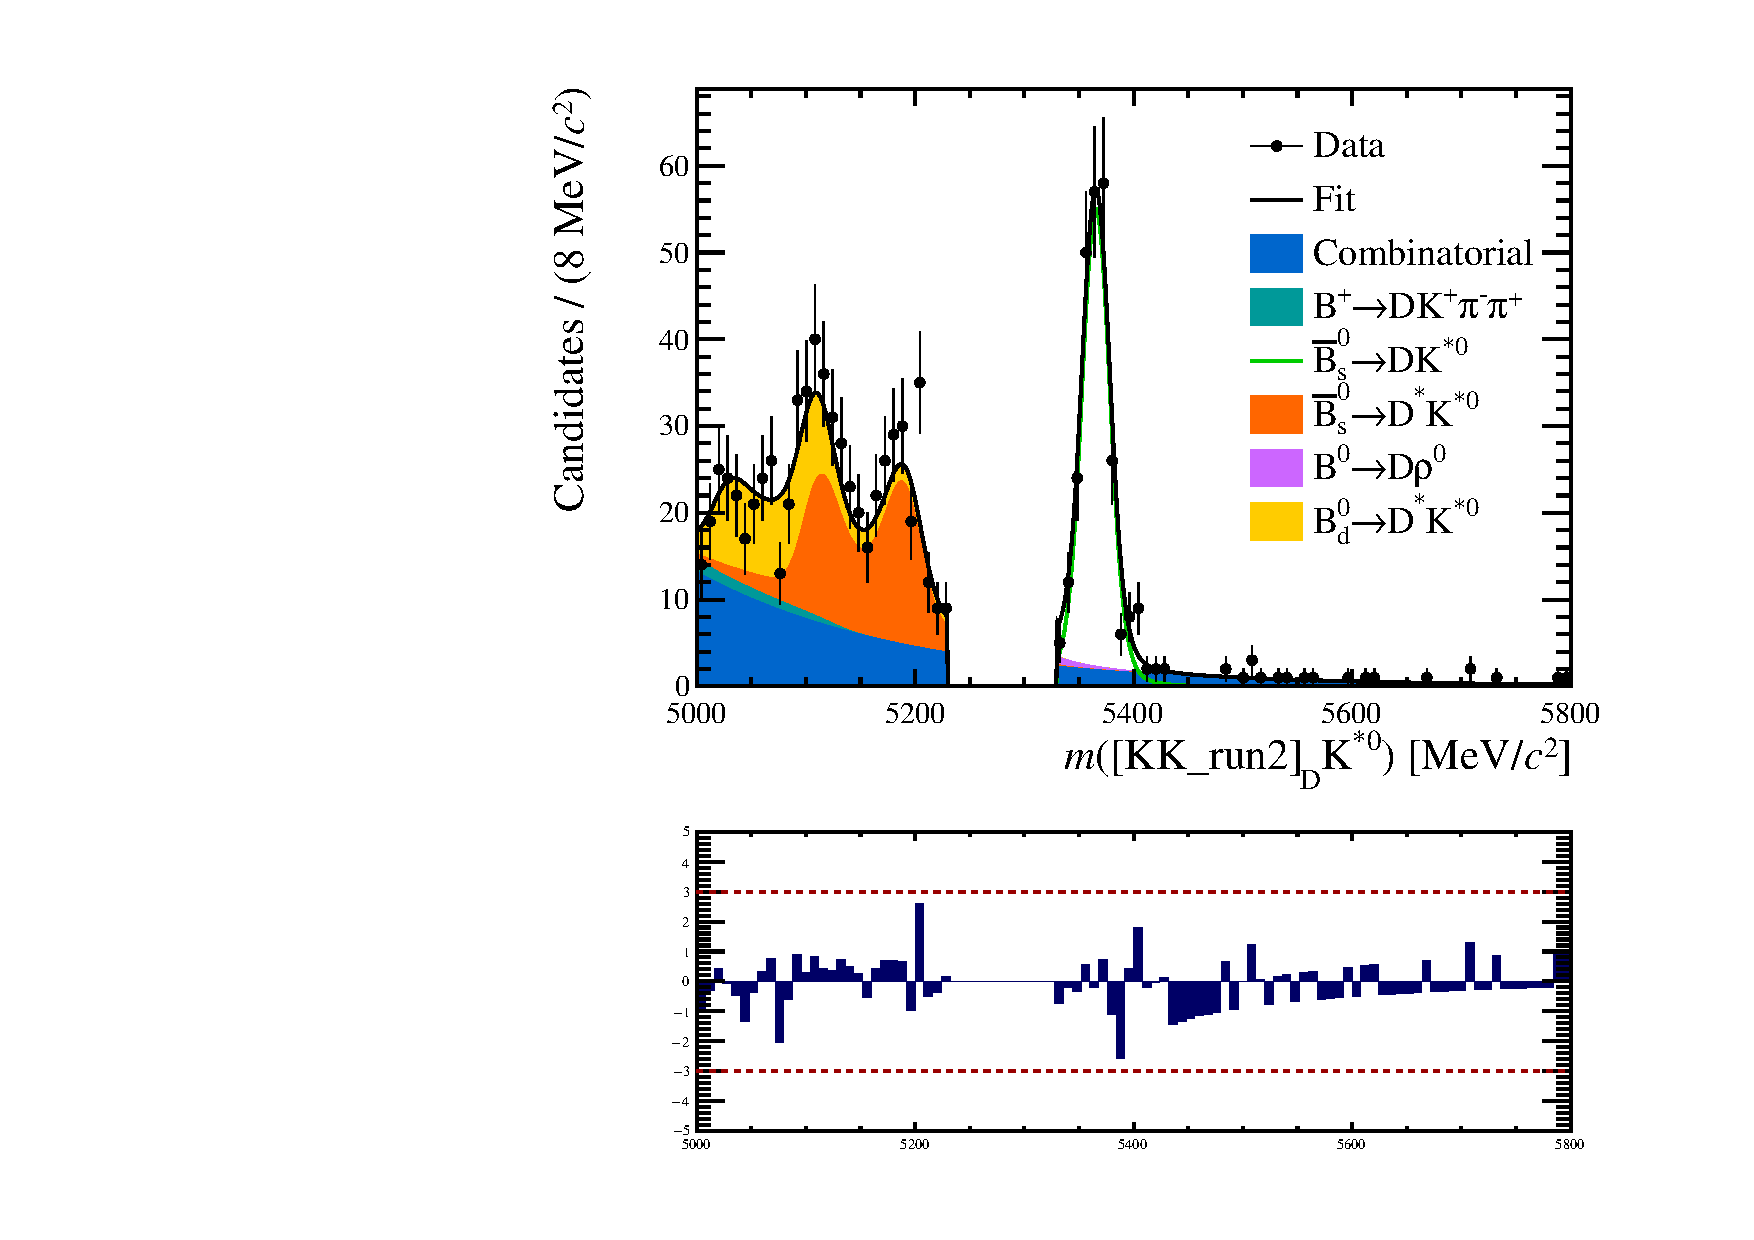
\includegraphics[width=0.45\textwidth]{ANA_resources/Plots/Data_fit/twoAndFourBody_data_KK_run2.pdf}} \\
    \end{tabular}
    \caption{Fit to $B$ invariant mass of selected candidates in the $KK$ final state, split by run and summed over $B$ flavour.}
\label{fig:data_fit_KK_combined}
\end{figure}
\begin{figure}[h]
    \centering
    \begin{tabular}{cc}
        \subfloat[][$B^0 \to D(\pi\pi)K^{*0}$ Run 1]{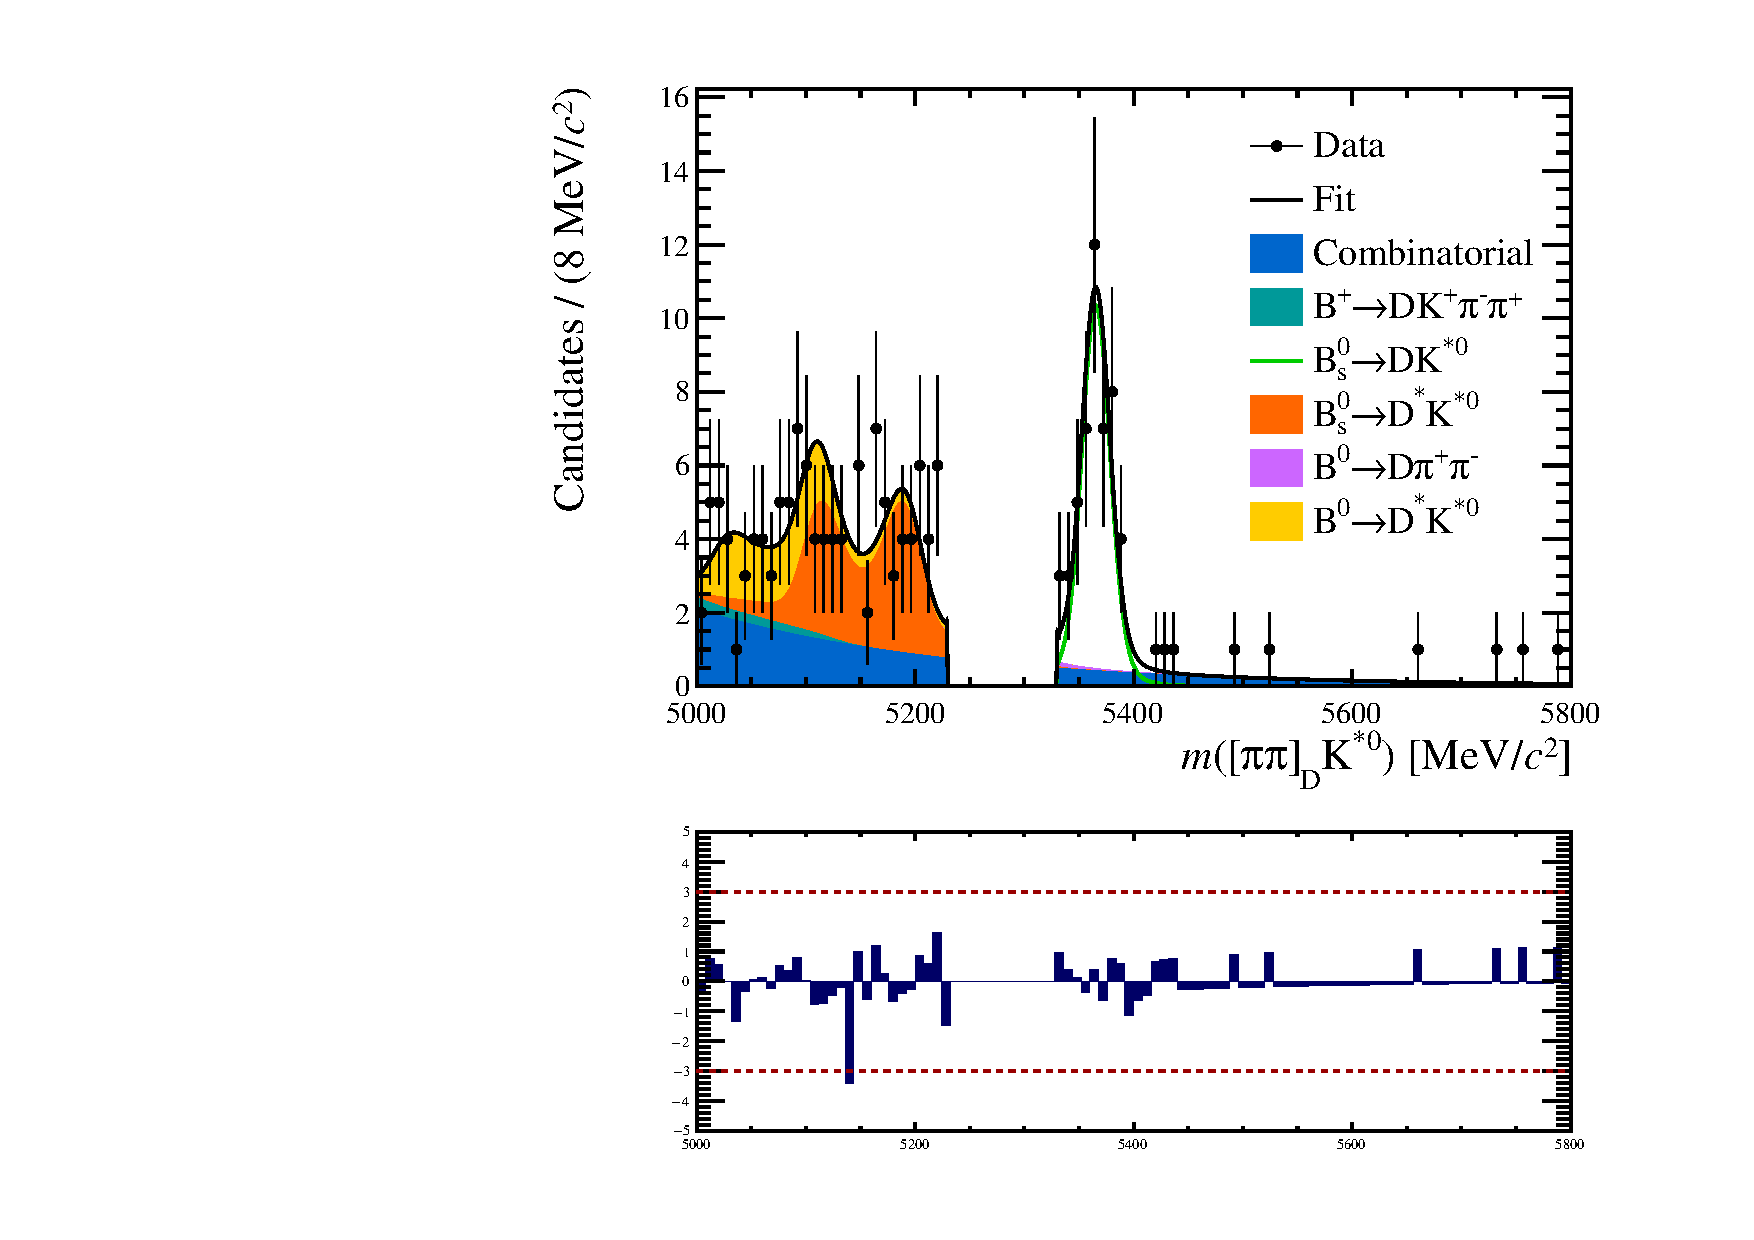
\includegraphics[width=0.45\textwidth]{ANA_resources/Plots/Data_fit/twoAndFourBody_data_pipi_run1}} &
        \subfloat[][$B^0 \to D(\pi\pi)K^{*0}$ Run 2]{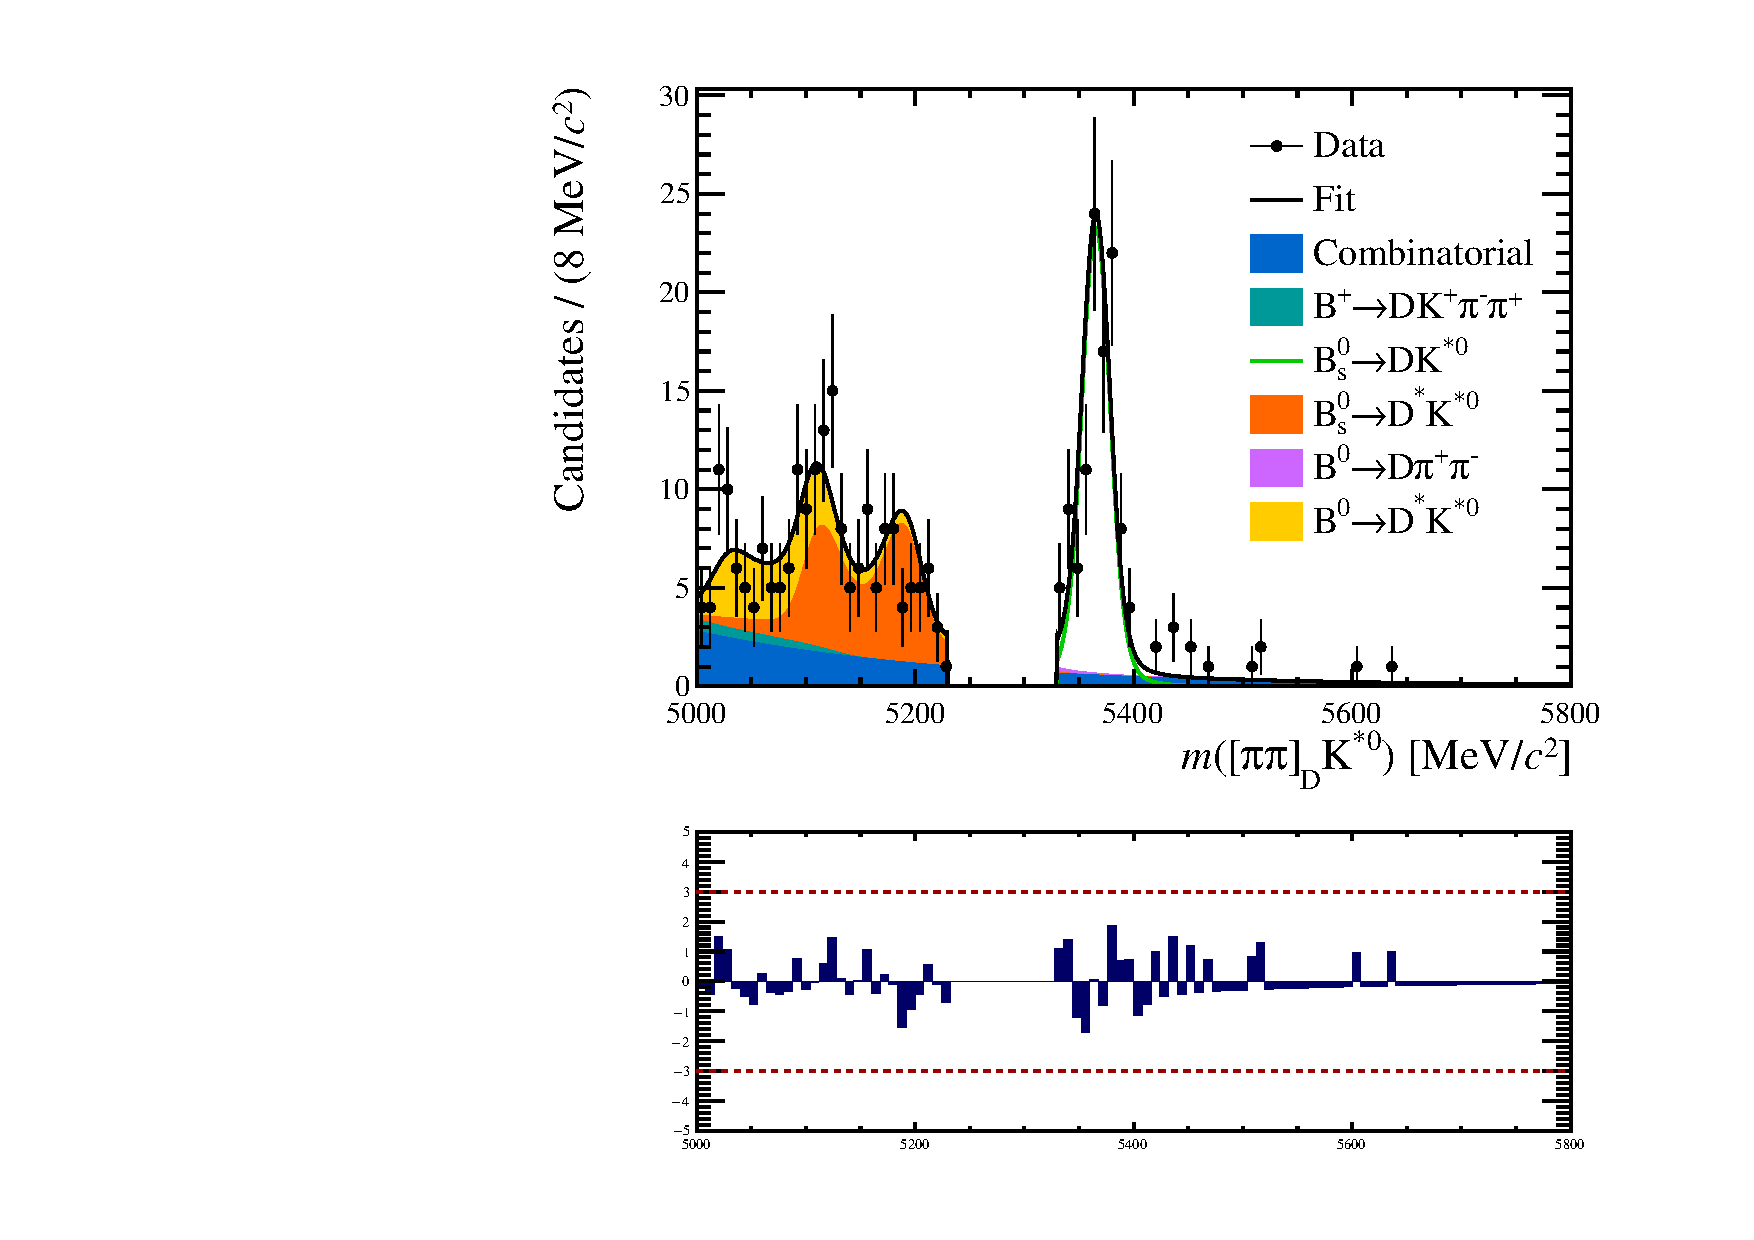
\includegraphics[width=0.45\textwidth]{ANA_resources/Plots/Data_fit/twoAndFourBody_data_pipi_run2.pdf}} \\
    \end{tabular}
    \caption{Fit to $B$ invariant mass of selected candidates in the $\pi\pi$ final state, split by run and summed over $B$ flavour.}
\label{fig:data_fit_pipi_combined}
\end{figure}
\begin{figure}[h]
    \centering
    \begin{tabular}{cc}
        \subfloat[][$B^0 \to D(K\pi\pi\pi)K^{*0}$ Run 1]{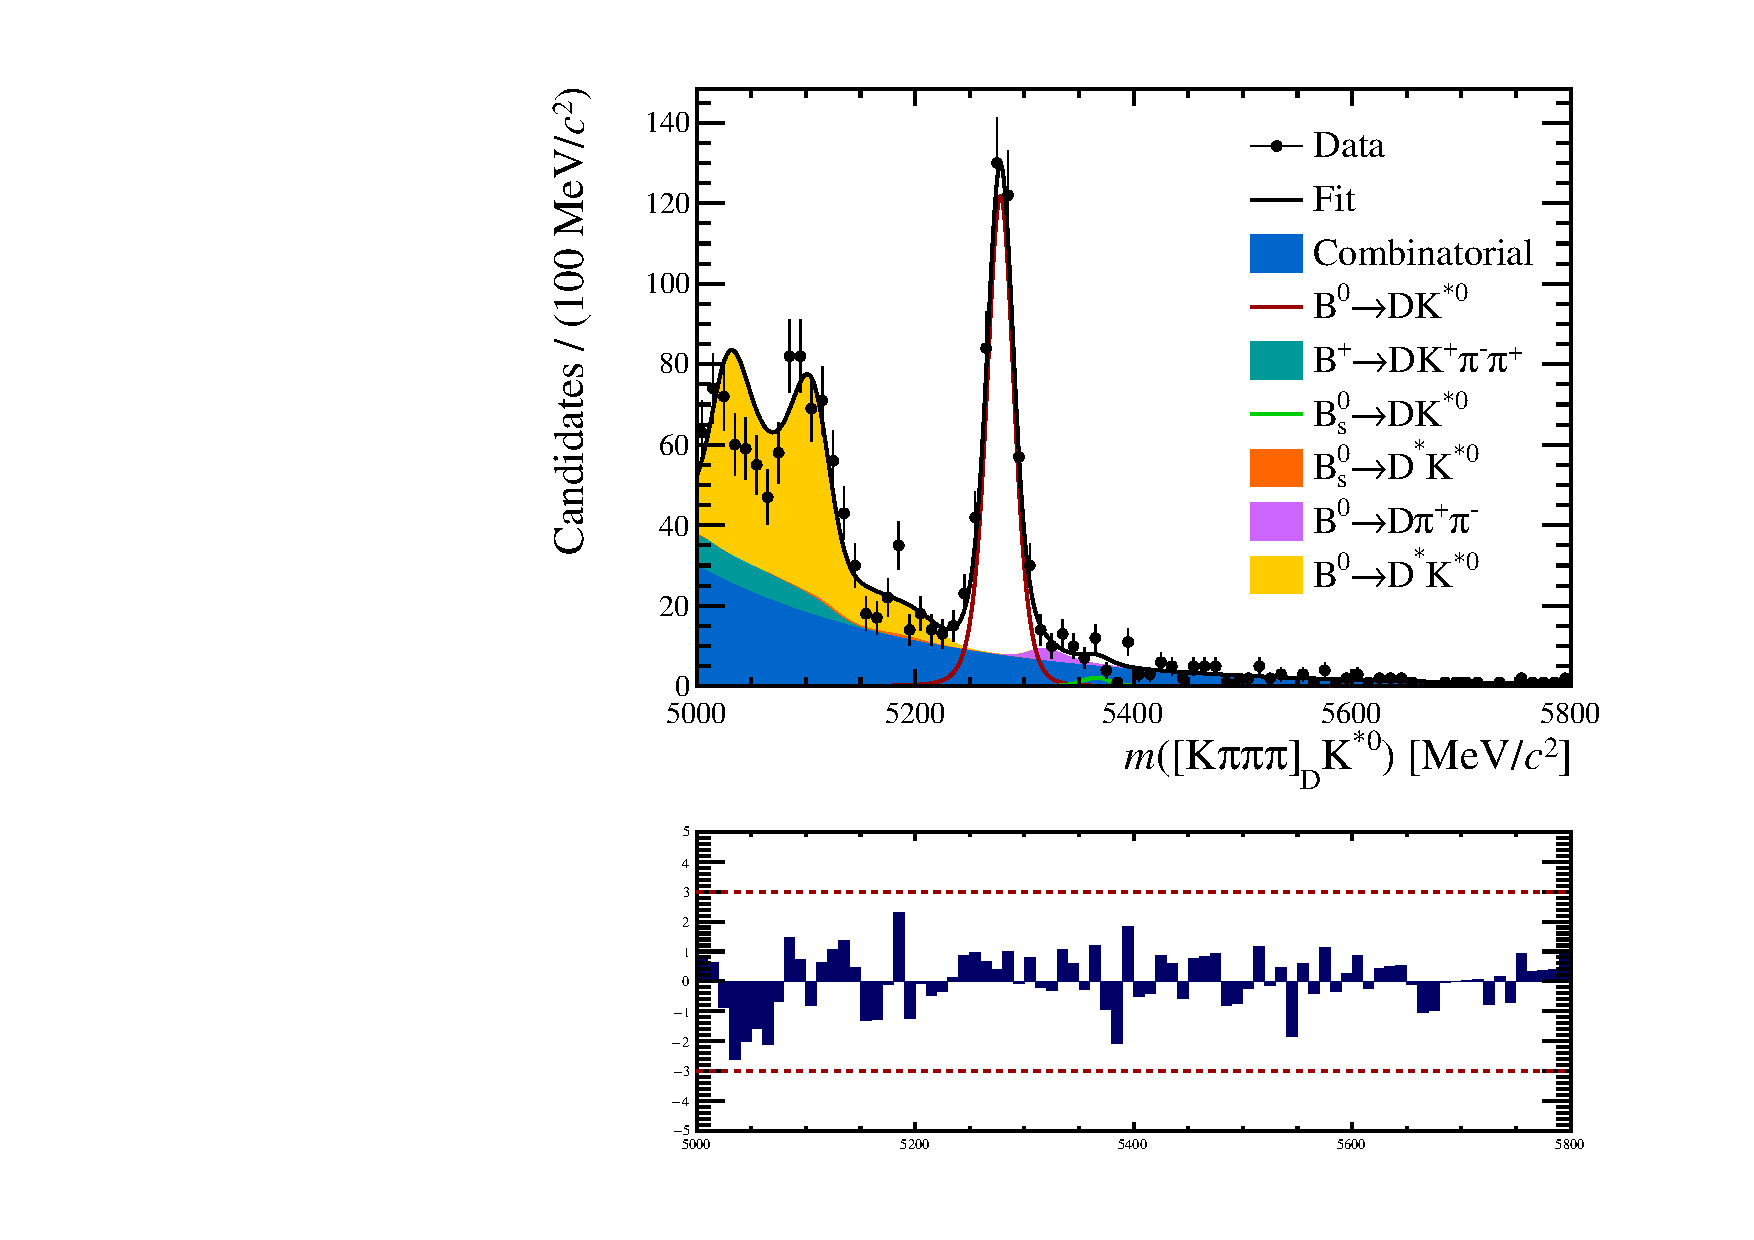
\includegraphics[width=0.45\textwidth]{ANA_resources/Plots/Data_fit/twoAndFourBody_data_Kpipipi_run1}} &
        \subfloat[][$B^0 \to D(K\pi\pi\pi)K^{*0}$ Run 2]{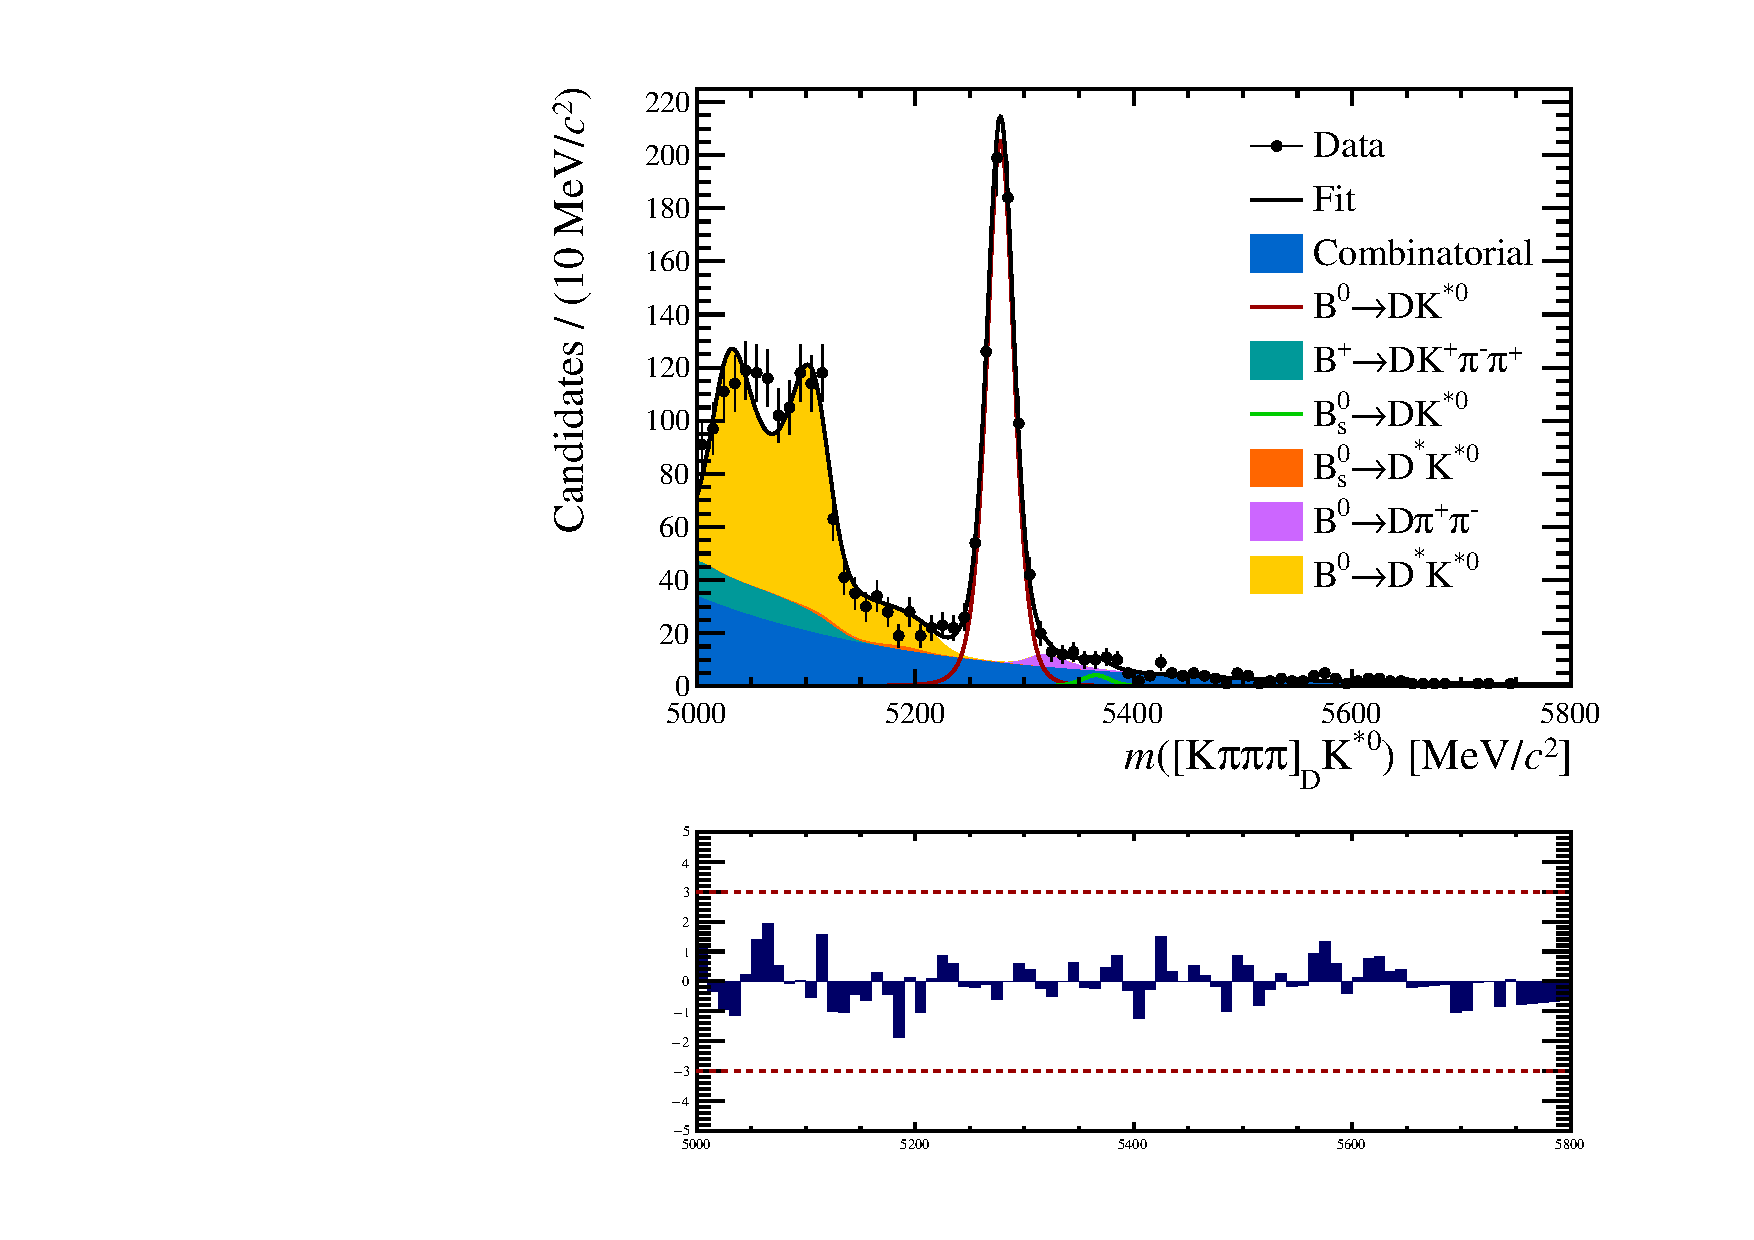
\includegraphics[width=0.45\textwidth]{ANA_resources/Plots/Data_fit/twoAndFourBody_data_Kpipipi_run2.pdf}} \\
    \end{tabular}
    \caption{Fit to $B$ invariant mass of selected candidates in the $K\pi\pi\pi$ final state, split by run and summed over $B$ flavour.}
\label{fig:data_fit_Kpipipi_combined}
\end{figure}
\begin{figure}[h]
    \centering
    \begin{tabular}{cc}
        \subfloat[][$B^0 \to D(\pi K\pi\pi)K^{*0}$ Run 1]{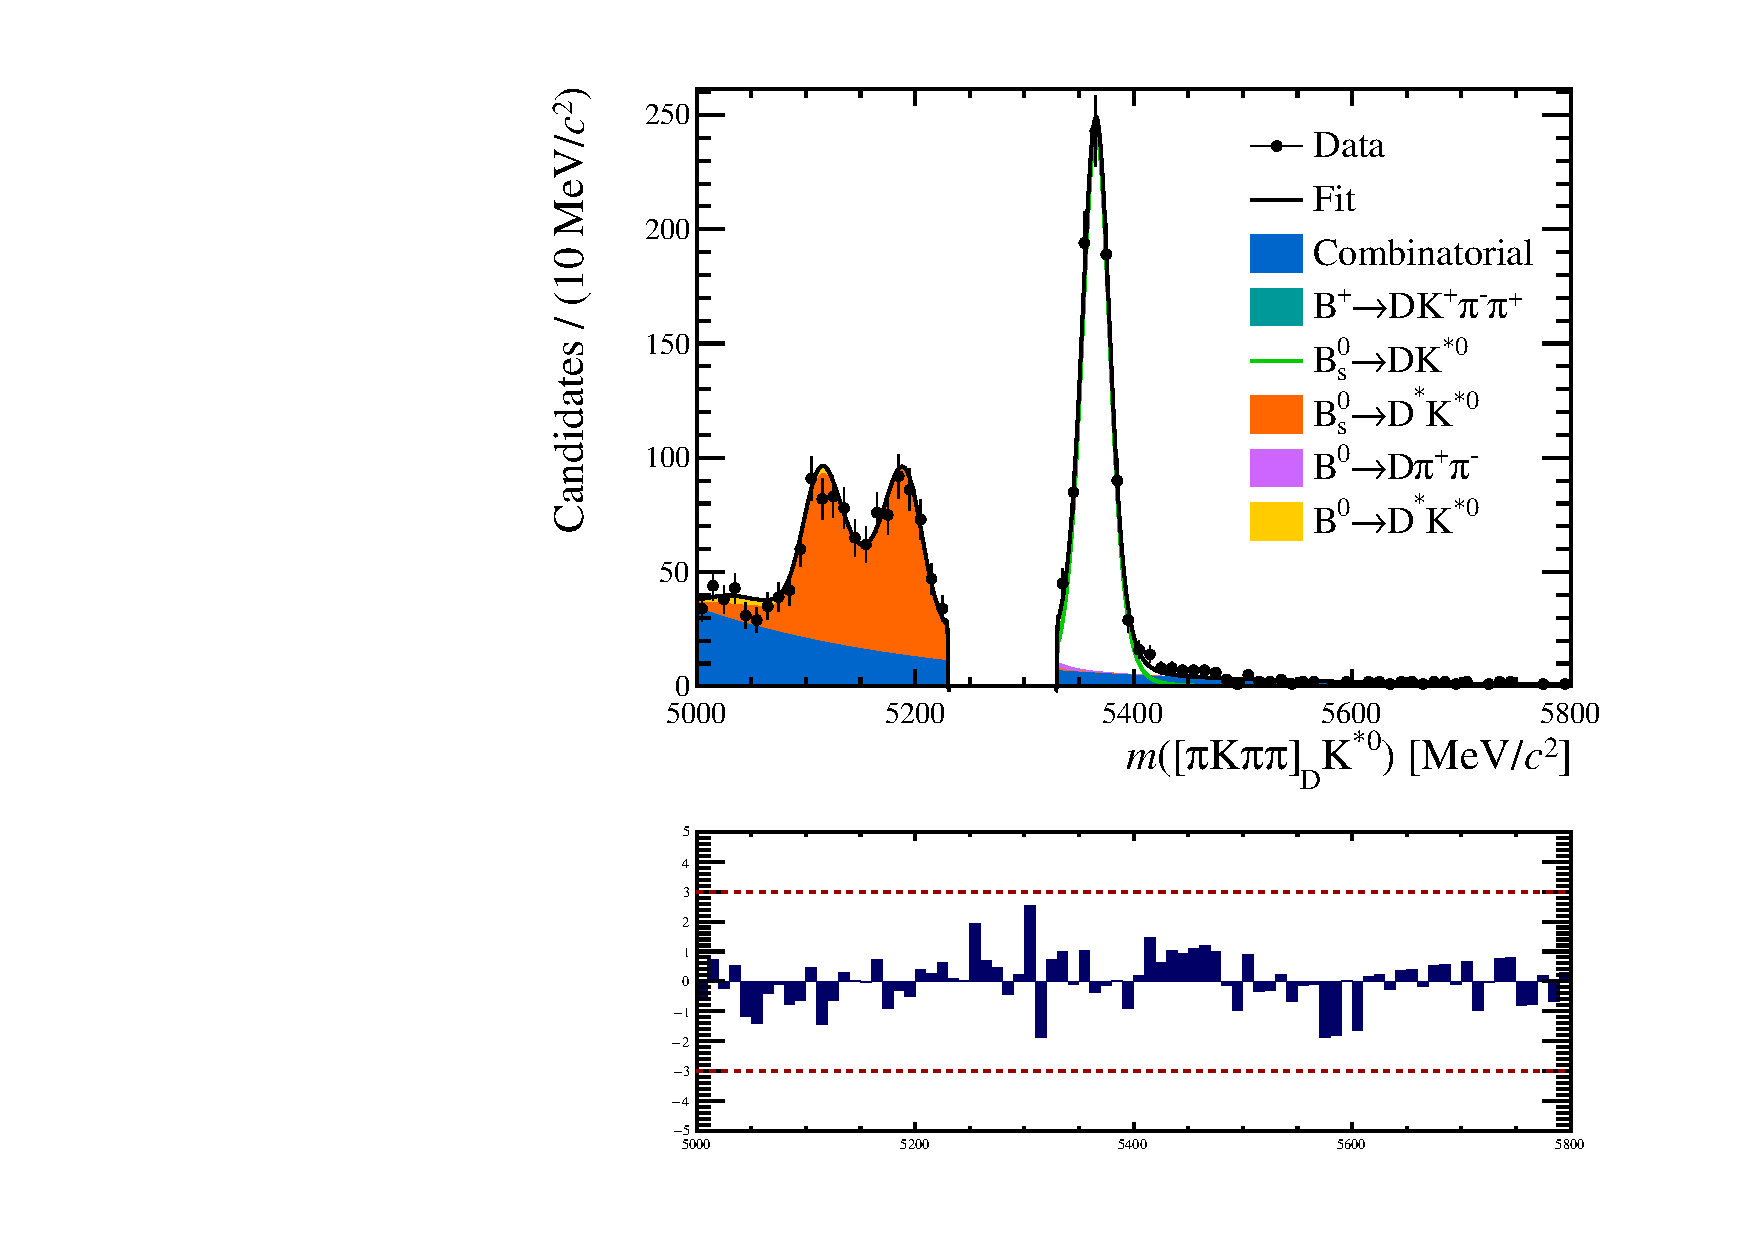
\includegraphics[width=0.45\textwidth]{ANA_resources/Plots/Data_fit/twoAndFourBody_data_piKpipi_run1}} &
        \subfloat[][$B^0 \to D(\pi K\pi\pi)K^{*0}$ Run 2]{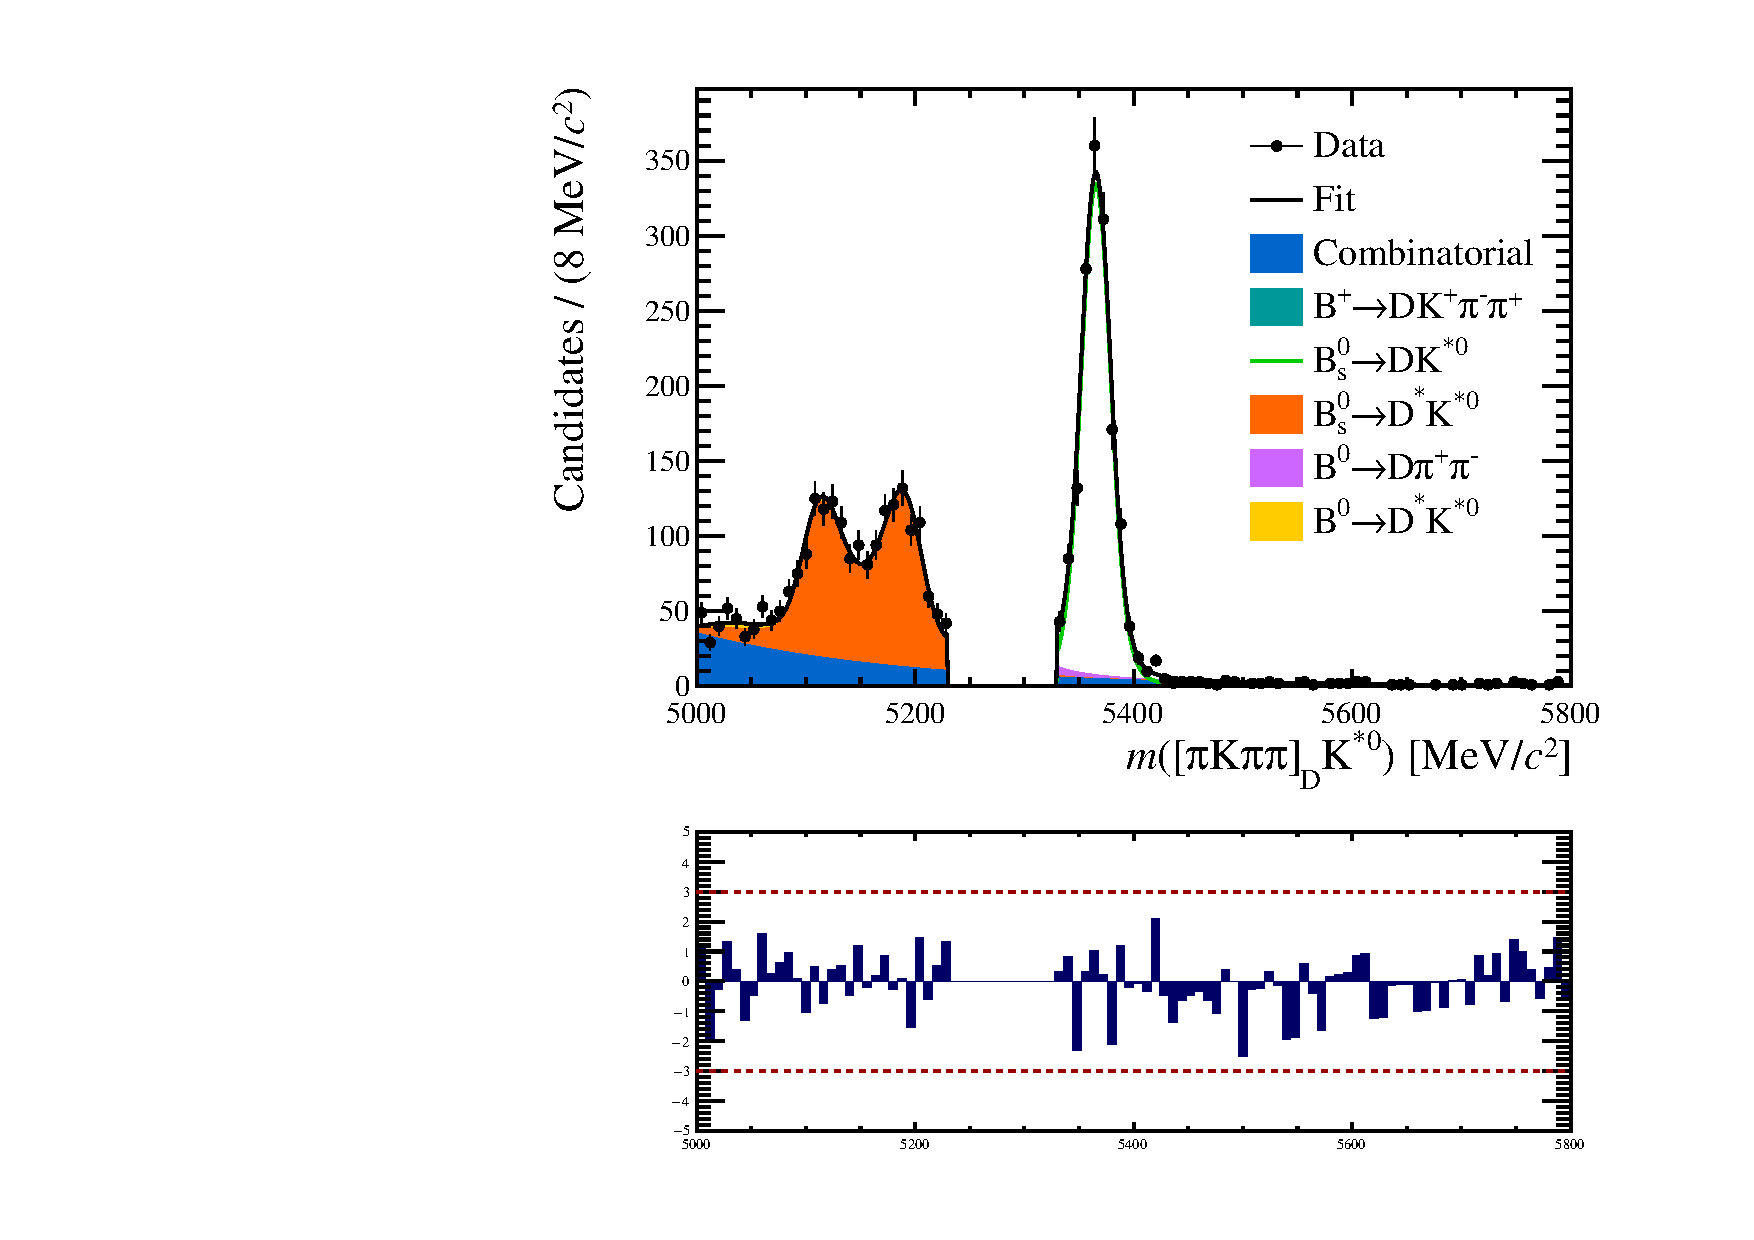
\includegraphics[width=0.45\textwidth]{ANA_resources/Plots/Data_fit/twoAndFourBody_data_piKpipi_run2.pdf}} \\
    \end{tabular}
    \caption{Fit to $B$ invariant mass of selected candidates in the $\pi K\pi\pi$ final state, split by run and summed over $B$ flavour.}
\label{fig:data_fit_piKpipi_combined}
\end{figure}
\begin{figure}[h]
    \centering
    \begin{tabular}{cc}
        \subfloat[][$B^0 \to D(\pi\pi\pi\pi)K^{*0}$ Run 2]{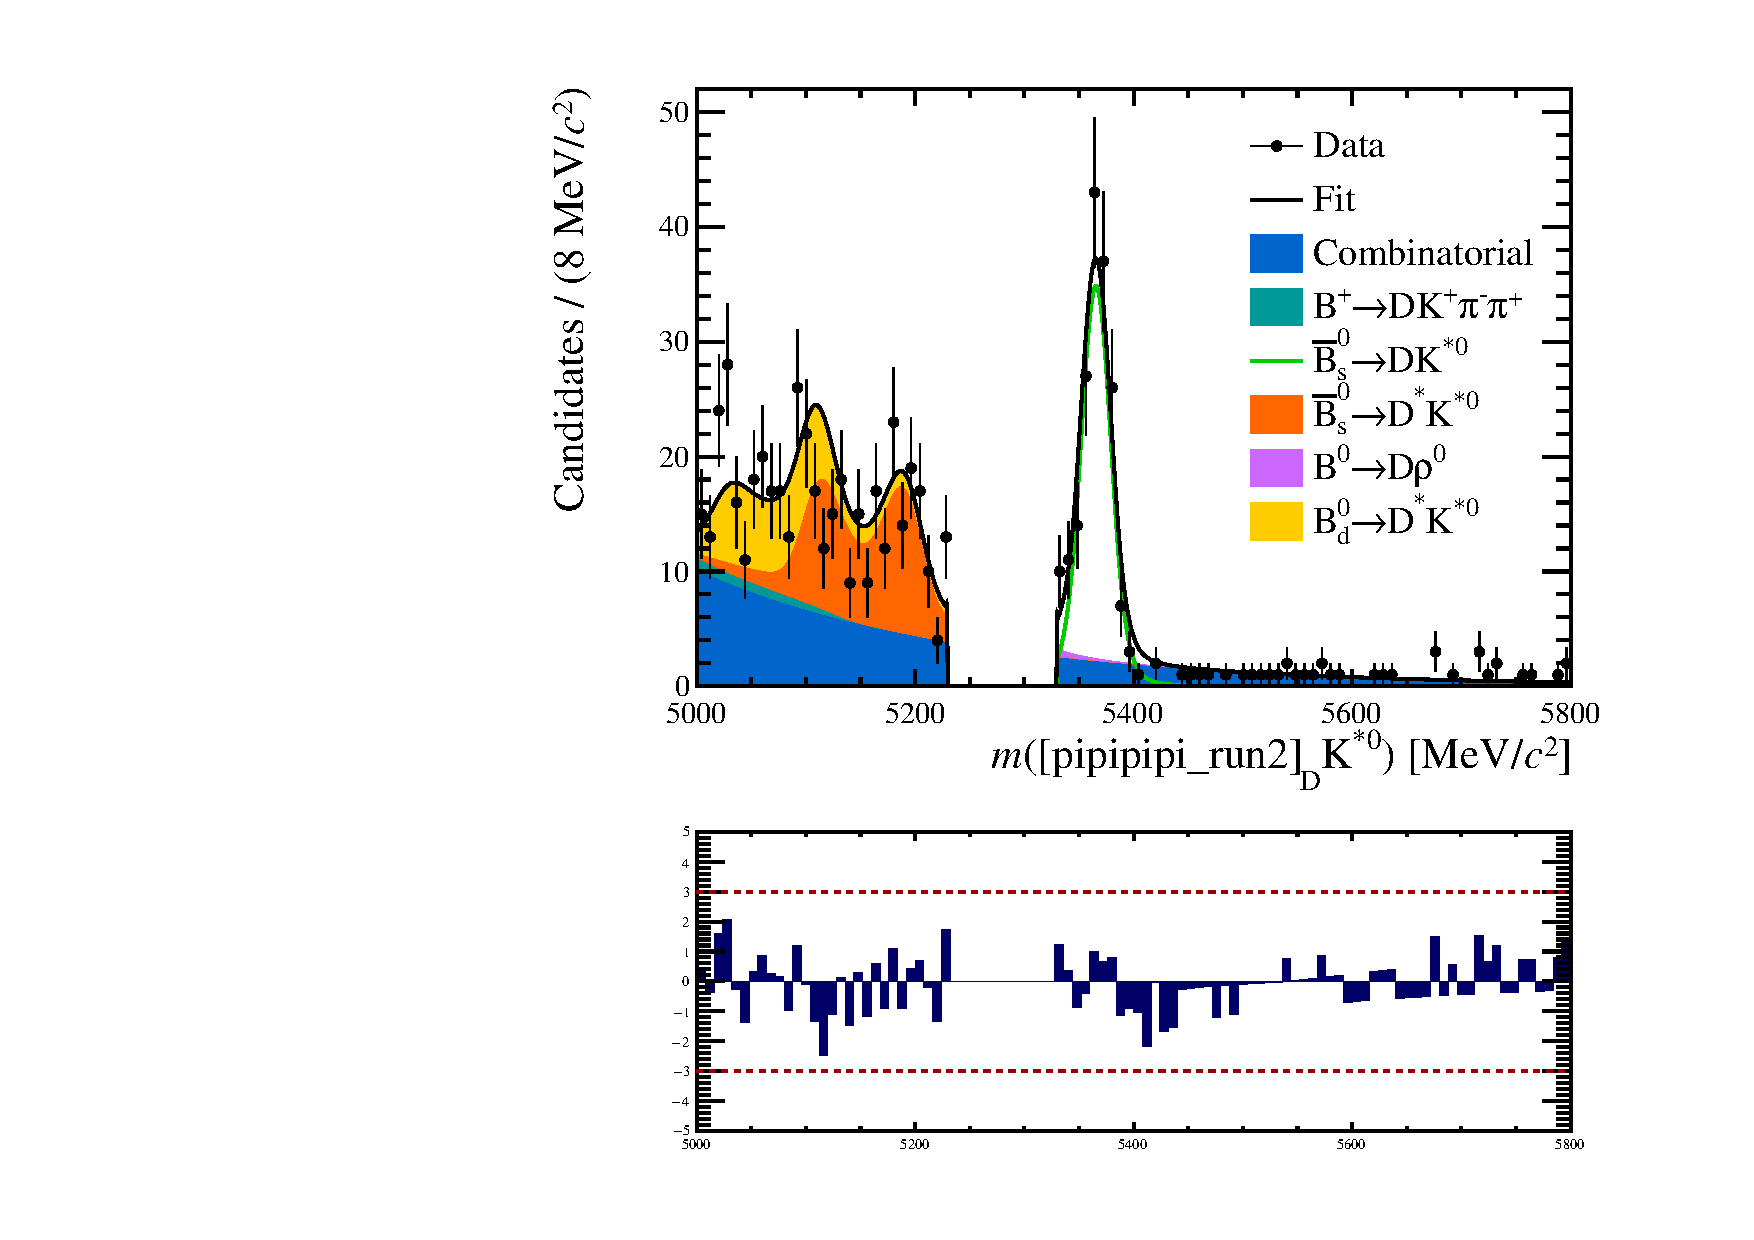
\includegraphics[width=0.45\textwidth]{ANA_resources/Plots/Data_fit/twoAndFourBody_data_pipipipi_run2.pdf}} \\
    \end{tabular}
    \caption{Fit to $B$ invariant mass of selected candidates in the $\pi\pi\pi\pi$ final state, split by run and summed over $B$ flavour.}
\label{fig:data_fit_pipipipi_combined}
\end{figure}
